
% Default to the notebook output style

    


% Inherit from the specified cell style.




    
\documentclass[11pt]{article}

    
    
    \usepackage[T1]{fontenc}
    % Nicer default font (+ math font) than Computer Modern for most use cases
    \usepackage{mathpazo}

    % Basic figure setup, for now with no caption control since it's done
    % automatically by Pandoc (which extracts ![](path) syntax from Markdown).
    \usepackage{graphicx}
    % We will generate all images so they have a width \maxwidth. This means
    % that they will get their normal width if they fit onto the page, but
    % are scaled down if they would overflow the margins.
    \makeatletter
    \def\maxwidth{\ifdim\Gin@nat@width>\linewidth\linewidth
    \else\Gin@nat@width\fi}
    \makeatother
    \let\Oldincludegraphics\includegraphics
    % Set max figure width to be 80% of text width, for now hardcoded.
    \renewcommand{\includegraphics}[1]{\Oldincludegraphics[width=.8\maxwidth]{#1}}
    % Ensure that by default, figures have no caption (until we provide a
    % proper Figure object with a Caption API and a way to capture that
    % in the conversion process - todo).
    \usepackage{caption}
    \DeclareCaptionLabelFormat{nolabel}{}
    \captionsetup{labelformat=nolabel}

    \usepackage{adjustbox} % Used to constrain images to a maximum size 
    \usepackage{xcolor} % Allow colors to be defined
    \usepackage{enumerate} % Needed for markdown enumerations to work
    \usepackage{geometry} % Used to adjust the document margins
    \usepackage{amsmath} % Equations
    \usepackage{amssymb} % Equations
    \usepackage{textcomp} % defines textquotesingle
    % Hack from http://tex.stackexchange.com/a/47451/13684:
    \AtBeginDocument{%
        \def\PYZsq{\textquotesingle}% Upright quotes in Pygmentized code
    }
    \usepackage{upquote} % Upright quotes for verbatim code
    \usepackage{eurosym} % defines \euro
    \usepackage[mathletters]{ucs} % Extended unicode (utf-8) support
    \usepackage[utf8x]{inputenc} % Allow utf-8 characters in the tex document
    \usepackage{fancyvrb} % verbatim replacement that allows latex
    \usepackage{grffile} % extends the file name processing of package graphics 
                         % to support a larger range 
    % The hyperref package gives us a pdf with properly built
    % internal navigation ('pdf bookmarks' for the table of contents,
    % internal cross-reference links, web links for URLs, etc.)
    \usepackage{hyperref}
    \usepackage{longtable} % longtable support required by pandoc >1.10
    \usepackage{booktabs}  % table support for pandoc > 1.12.2
    \usepackage[inline]{enumitem} % IRkernel/repr support (it uses the enumerate* environment)
    \usepackage[normalem]{ulem} % ulem is needed to support strikethroughs (\sout)
                                % normalem makes italics be italics, not underlines
    

    
    
    % Colors for the hyperref package
    \definecolor{urlcolor}{rgb}{0,.145,.698}
    \definecolor{linkcolor}{rgb}{.71,0.21,0.01}
    \definecolor{citecolor}{rgb}{.12,.54,.11}

    % ANSI colors
    \definecolor{ansi-black}{HTML}{3E424D}
    \definecolor{ansi-black-intense}{HTML}{282C36}
    \definecolor{ansi-red}{HTML}{E75C58}
    \definecolor{ansi-red-intense}{HTML}{B22B31}
    \definecolor{ansi-green}{HTML}{00A250}
    \definecolor{ansi-green-intense}{HTML}{007427}
    \definecolor{ansi-yellow}{HTML}{DDB62B}
    \definecolor{ansi-yellow-intense}{HTML}{B27D12}
    \definecolor{ansi-blue}{HTML}{208FFB}
    \definecolor{ansi-blue-intense}{HTML}{0065CA}
    \definecolor{ansi-magenta}{HTML}{D160C4}
    \definecolor{ansi-magenta-intense}{HTML}{A03196}
    \definecolor{ansi-cyan}{HTML}{60C6C8}
    \definecolor{ansi-cyan-intense}{HTML}{258F8F}
    \definecolor{ansi-white}{HTML}{C5C1B4}
    \definecolor{ansi-white-intense}{HTML}{A1A6B2}

    % commands and environments needed by pandoc snippets
    % extracted from the output of `pandoc -s`
    \providecommand{\tightlist}{%
      \setlength{\itemsep}{0pt}\setlength{\parskip}{0pt}}
    \DefineVerbatimEnvironment{Highlighting}{Verbatim}{commandchars=\\\{\}}
    % Add ',fontsize=\small' for more characters per line
    \newenvironment{Shaded}{}{}
    \newcommand{\KeywordTok}[1]{\textcolor[rgb]{0.00,0.44,0.13}{\textbf{{#1}}}}
    \newcommand{\DataTypeTok}[1]{\textcolor[rgb]{0.56,0.13,0.00}{{#1}}}
    \newcommand{\DecValTok}[1]{\textcolor[rgb]{0.25,0.63,0.44}{{#1}}}
    \newcommand{\BaseNTok}[1]{\textcolor[rgb]{0.25,0.63,0.44}{{#1}}}
    \newcommand{\FloatTok}[1]{\textcolor[rgb]{0.25,0.63,0.44}{{#1}}}
    \newcommand{\CharTok}[1]{\textcolor[rgb]{0.25,0.44,0.63}{{#1}}}
    \newcommand{\StringTok}[1]{\textcolor[rgb]{0.25,0.44,0.63}{{#1}}}
    \newcommand{\CommentTok}[1]{\textcolor[rgb]{0.38,0.63,0.69}{\textit{{#1}}}}
    \newcommand{\OtherTok}[1]{\textcolor[rgb]{0.00,0.44,0.13}{{#1}}}
    \newcommand{\AlertTok}[1]{\textcolor[rgb]{1.00,0.00,0.00}{\textbf{{#1}}}}
    \newcommand{\FunctionTok}[1]{\textcolor[rgb]{0.02,0.16,0.49}{{#1}}}
    \newcommand{\RegionMarkerTok}[1]{{#1}}
    \newcommand{\ErrorTok}[1]{\textcolor[rgb]{1.00,0.00,0.00}{\textbf{{#1}}}}
    \newcommand{\NormalTok}[1]{{#1}}
    
    % Additional commands for more recent versions of Pandoc
    \newcommand{\ConstantTok}[1]{\textcolor[rgb]{0.53,0.00,0.00}{{#1}}}
    \newcommand{\SpecialCharTok}[1]{\textcolor[rgb]{0.25,0.44,0.63}{{#1}}}
    \newcommand{\VerbatimStringTok}[1]{\textcolor[rgb]{0.25,0.44,0.63}{{#1}}}
    \newcommand{\SpecialStringTok}[1]{\textcolor[rgb]{0.73,0.40,0.53}{{#1}}}
    \newcommand{\ImportTok}[1]{{#1}}
    \newcommand{\DocumentationTok}[1]{\textcolor[rgb]{0.73,0.13,0.13}{\textit{{#1}}}}
    \newcommand{\AnnotationTok}[1]{\textcolor[rgb]{0.38,0.63,0.69}{\textbf{\textit{{#1}}}}}
    \newcommand{\CommentVarTok}[1]{\textcolor[rgb]{0.38,0.63,0.69}{\textbf{\textit{{#1}}}}}
    \newcommand{\VariableTok}[1]{\textcolor[rgb]{0.10,0.09,0.49}{{#1}}}
    \newcommand{\ControlFlowTok}[1]{\textcolor[rgb]{0.00,0.44,0.13}{\textbf{{#1}}}}
    \newcommand{\OperatorTok}[1]{\textcolor[rgb]{0.40,0.40,0.40}{{#1}}}
    \newcommand{\BuiltInTok}[1]{{#1}}
    \newcommand{\ExtensionTok}[1]{{#1}}
    \newcommand{\PreprocessorTok}[1]{\textcolor[rgb]{0.74,0.48,0.00}{{#1}}}
    \newcommand{\AttributeTok}[1]{\textcolor[rgb]{0.49,0.56,0.16}{{#1}}}
    \newcommand{\InformationTok}[1]{\textcolor[rgb]{0.38,0.63,0.69}{\textbf{\textit{{#1}}}}}
    \newcommand{\WarningTok}[1]{\textcolor[rgb]{0.38,0.63,0.69}{\textbf{\textit{{#1}}}}}
    
    
    % Define a nice break command that doesn't care if a line doesn't already
    % exist.
    \def\br{\hspace*{\fill} \\* }
    % Math Jax compatability definitions
    \def\gt{>}
    \def\lt{<}
    % Document parameters
    \title{Recursi?n\_Backtracking}
    
    
    

    % Pygments definitions
    
\makeatletter
\def\PY@reset{\let\PY@it=\relax \let\PY@bf=\relax%
    \let\PY@ul=\relax \let\PY@tc=\relax%
    \let\PY@bc=\relax \let\PY@ff=\relax}
\def\PY@tok#1{\csname PY@tok@#1\endcsname}
\def\PY@toks#1+{\ifx\relax#1\empty\else%
    \PY@tok{#1}\expandafter\PY@toks\fi}
\def\PY@do#1{\PY@bc{\PY@tc{\PY@ul{%
    \PY@it{\PY@bf{\PY@ff{#1}}}}}}}
\def\PY#1#2{\PY@reset\PY@toks#1+\relax+\PY@do{#2}}

\expandafter\def\csname PY@tok@w\endcsname{\def\PY@tc##1{\textcolor[rgb]{0.73,0.73,0.73}{##1}}}
\expandafter\def\csname PY@tok@c\endcsname{\let\PY@it=\textit\def\PY@tc##1{\textcolor[rgb]{0.25,0.50,0.50}{##1}}}
\expandafter\def\csname PY@tok@cp\endcsname{\def\PY@tc##1{\textcolor[rgb]{0.74,0.48,0.00}{##1}}}
\expandafter\def\csname PY@tok@k\endcsname{\let\PY@bf=\textbf\def\PY@tc##1{\textcolor[rgb]{0.00,0.50,0.00}{##1}}}
\expandafter\def\csname PY@tok@kp\endcsname{\def\PY@tc##1{\textcolor[rgb]{0.00,0.50,0.00}{##1}}}
\expandafter\def\csname PY@tok@kt\endcsname{\def\PY@tc##1{\textcolor[rgb]{0.69,0.00,0.25}{##1}}}
\expandafter\def\csname PY@tok@o\endcsname{\def\PY@tc##1{\textcolor[rgb]{0.40,0.40,0.40}{##1}}}
\expandafter\def\csname PY@tok@ow\endcsname{\let\PY@bf=\textbf\def\PY@tc##1{\textcolor[rgb]{0.67,0.13,1.00}{##1}}}
\expandafter\def\csname PY@tok@nb\endcsname{\def\PY@tc##1{\textcolor[rgb]{0.00,0.50,0.00}{##1}}}
\expandafter\def\csname PY@tok@nf\endcsname{\def\PY@tc##1{\textcolor[rgb]{0.00,0.00,1.00}{##1}}}
\expandafter\def\csname PY@tok@nc\endcsname{\let\PY@bf=\textbf\def\PY@tc##1{\textcolor[rgb]{0.00,0.00,1.00}{##1}}}
\expandafter\def\csname PY@tok@nn\endcsname{\let\PY@bf=\textbf\def\PY@tc##1{\textcolor[rgb]{0.00,0.00,1.00}{##1}}}
\expandafter\def\csname PY@tok@ne\endcsname{\let\PY@bf=\textbf\def\PY@tc##1{\textcolor[rgb]{0.82,0.25,0.23}{##1}}}
\expandafter\def\csname PY@tok@nv\endcsname{\def\PY@tc##1{\textcolor[rgb]{0.10,0.09,0.49}{##1}}}
\expandafter\def\csname PY@tok@no\endcsname{\def\PY@tc##1{\textcolor[rgb]{0.53,0.00,0.00}{##1}}}
\expandafter\def\csname PY@tok@nl\endcsname{\def\PY@tc##1{\textcolor[rgb]{0.63,0.63,0.00}{##1}}}
\expandafter\def\csname PY@tok@ni\endcsname{\let\PY@bf=\textbf\def\PY@tc##1{\textcolor[rgb]{0.60,0.60,0.60}{##1}}}
\expandafter\def\csname PY@tok@na\endcsname{\def\PY@tc##1{\textcolor[rgb]{0.49,0.56,0.16}{##1}}}
\expandafter\def\csname PY@tok@nt\endcsname{\let\PY@bf=\textbf\def\PY@tc##1{\textcolor[rgb]{0.00,0.50,0.00}{##1}}}
\expandafter\def\csname PY@tok@nd\endcsname{\def\PY@tc##1{\textcolor[rgb]{0.67,0.13,1.00}{##1}}}
\expandafter\def\csname PY@tok@s\endcsname{\def\PY@tc##1{\textcolor[rgb]{0.73,0.13,0.13}{##1}}}
\expandafter\def\csname PY@tok@sd\endcsname{\let\PY@it=\textit\def\PY@tc##1{\textcolor[rgb]{0.73,0.13,0.13}{##1}}}
\expandafter\def\csname PY@tok@si\endcsname{\let\PY@bf=\textbf\def\PY@tc##1{\textcolor[rgb]{0.73,0.40,0.53}{##1}}}
\expandafter\def\csname PY@tok@se\endcsname{\let\PY@bf=\textbf\def\PY@tc##1{\textcolor[rgb]{0.73,0.40,0.13}{##1}}}
\expandafter\def\csname PY@tok@sr\endcsname{\def\PY@tc##1{\textcolor[rgb]{0.73,0.40,0.53}{##1}}}
\expandafter\def\csname PY@tok@ss\endcsname{\def\PY@tc##1{\textcolor[rgb]{0.10,0.09,0.49}{##1}}}
\expandafter\def\csname PY@tok@sx\endcsname{\def\PY@tc##1{\textcolor[rgb]{0.00,0.50,0.00}{##1}}}
\expandafter\def\csname PY@tok@m\endcsname{\def\PY@tc##1{\textcolor[rgb]{0.40,0.40,0.40}{##1}}}
\expandafter\def\csname PY@tok@gh\endcsname{\let\PY@bf=\textbf\def\PY@tc##1{\textcolor[rgb]{0.00,0.00,0.50}{##1}}}
\expandafter\def\csname PY@tok@gu\endcsname{\let\PY@bf=\textbf\def\PY@tc##1{\textcolor[rgb]{0.50,0.00,0.50}{##1}}}
\expandafter\def\csname PY@tok@gd\endcsname{\def\PY@tc##1{\textcolor[rgb]{0.63,0.00,0.00}{##1}}}
\expandafter\def\csname PY@tok@gi\endcsname{\def\PY@tc##1{\textcolor[rgb]{0.00,0.63,0.00}{##1}}}
\expandafter\def\csname PY@tok@gr\endcsname{\def\PY@tc##1{\textcolor[rgb]{1.00,0.00,0.00}{##1}}}
\expandafter\def\csname PY@tok@ge\endcsname{\let\PY@it=\textit}
\expandafter\def\csname PY@tok@gs\endcsname{\let\PY@bf=\textbf}
\expandafter\def\csname PY@tok@gp\endcsname{\let\PY@bf=\textbf\def\PY@tc##1{\textcolor[rgb]{0.00,0.00,0.50}{##1}}}
\expandafter\def\csname PY@tok@go\endcsname{\def\PY@tc##1{\textcolor[rgb]{0.53,0.53,0.53}{##1}}}
\expandafter\def\csname PY@tok@gt\endcsname{\def\PY@tc##1{\textcolor[rgb]{0.00,0.27,0.87}{##1}}}
\expandafter\def\csname PY@tok@err\endcsname{\def\PY@bc##1{\setlength{\fboxsep}{0pt}\fcolorbox[rgb]{1.00,0.00,0.00}{1,1,1}{\strut ##1}}}
\expandafter\def\csname PY@tok@kc\endcsname{\let\PY@bf=\textbf\def\PY@tc##1{\textcolor[rgb]{0.00,0.50,0.00}{##1}}}
\expandafter\def\csname PY@tok@kd\endcsname{\let\PY@bf=\textbf\def\PY@tc##1{\textcolor[rgb]{0.00,0.50,0.00}{##1}}}
\expandafter\def\csname PY@tok@kn\endcsname{\let\PY@bf=\textbf\def\PY@tc##1{\textcolor[rgb]{0.00,0.50,0.00}{##1}}}
\expandafter\def\csname PY@tok@kr\endcsname{\let\PY@bf=\textbf\def\PY@tc##1{\textcolor[rgb]{0.00,0.50,0.00}{##1}}}
\expandafter\def\csname PY@tok@bp\endcsname{\def\PY@tc##1{\textcolor[rgb]{0.00,0.50,0.00}{##1}}}
\expandafter\def\csname PY@tok@fm\endcsname{\def\PY@tc##1{\textcolor[rgb]{0.00,0.00,1.00}{##1}}}
\expandafter\def\csname PY@tok@vc\endcsname{\def\PY@tc##1{\textcolor[rgb]{0.10,0.09,0.49}{##1}}}
\expandafter\def\csname PY@tok@vg\endcsname{\def\PY@tc##1{\textcolor[rgb]{0.10,0.09,0.49}{##1}}}
\expandafter\def\csname PY@tok@vi\endcsname{\def\PY@tc##1{\textcolor[rgb]{0.10,0.09,0.49}{##1}}}
\expandafter\def\csname PY@tok@vm\endcsname{\def\PY@tc##1{\textcolor[rgb]{0.10,0.09,0.49}{##1}}}
\expandafter\def\csname PY@tok@sa\endcsname{\def\PY@tc##1{\textcolor[rgb]{0.73,0.13,0.13}{##1}}}
\expandafter\def\csname PY@tok@sb\endcsname{\def\PY@tc##1{\textcolor[rgb]{0.73,0.13,0.13}{##1}}}
\expandafter\def\csname PY@tok@sc\endcsname{\def\PY@tc##1{\textcolor[rgb]{0.73,0.13,0.13}{##1}}}
\expandafter\def\csname PY@tok@dl\endcsname{\def\PY@tc##1{\textcolor[rgb]{0.73,0.13,0.13}{##1}}}
\expandafter\def\csname PY@tok@s2\endcsname{\def\PY@tc##1{\textcolor[rgb]{0.73,0.13,0.13}{##1}}}
\expandafter\def\csname PY@tok@sh\endcsname{\def\PY@tc##1{\textcolor[rgb]{0.73,0.13,0.13}{##1}}}
\expandafter\def\csname PY@tok@s1\endcsname{\def\PY@tc##1{\textcolor[rgb]{0.73,0.13,0.13}{##1}}}
\expandafter\def\csname PY@tok@mb\endcsname{\def\PY@tc##1{\textcolor[rgb]{0.40,0.40,0.40}{##1}}}
\expandafter\def\csname PY@tok@mf\endcsname{\def\PY@tc##1{\textcolor[rgb]{0.40,0.40,0.40}{##1}}}
\expandafter\def\csname PY@tok@mh\endcsname{\def\PY@tc##1{\textcolor[rgb]{0.40,0.40,0.40}{##1}}}
\expandafter\def\csname PY@tok@mi\endcsname{\def\PY@tc##1{\textcolor[rgb]{0.40,0.40,0.40}{##1}}}
\expandafter\def\csname PY@tok@il\endcsname{\def\PY@tc##1{\textcolor[rgb]{0.40,0.40,0.40}{##1}}}
\expandafter\def\csname PY@tok@mo\endcsname{\def\PY@tc##1{\textcolor[rgb]{0.40,0.40,0.40}{##1}}}
\expandafter\def\csname PY@tok@ch\endcsname{\let\PY@it=\textit\def\PY@tc##1{\textcolor[rgb]{0.25,0.50,0.50}{##1}}}
\expandafter\def\csname PY@tok@cm\endcsname{\let\PY@it=\textit\def\PY@tc##1{\textcolor[rgb]{0.25,0.50,0.50}{##1}}}
\expandafter\def\csname PY@tok@cpf\endcsname{\let\PY@it=\textit\def\PY@tc##1{\textcolor[rgb]{0.25,0.50,0.50}{##1}}}
\expandafter\def\csname PY@tok@c1\endcsname{\let\PY@it=\textit\def\PY@tc##1{\textcolor[rgb]{0.25,0.50,0.50}{##1}}}
\expandafter\def\csname PY@tok@cs\endcsname{\let\PY@it=\textit\def\PY@tc##1{\textcolor[rgb]{0.25,0.50,0.50}{##1}}}

\def\PYZbs{\char`\\}
\def\PYZus{\char`\_}
\def\PYZob{\char`\{}
\def\PYZcb{\char`\}}
\def\PYZca{\char`\^}
\def\PYZam{\char`\&}
\def\PYZlt{\char`\<}
\def\PYZgt{\char`\>}
\def\PYZsh{\char`\#}
\def\PYZpc{\char`\%}
\def\PYZdl{\char`\$}
\def\PYZhy{\char`\-}
\def\PYZsq{\char`\'}
\def\PYZdq{\char`\"}
\def\PYZti{\char`\~}
% for compatibility with earlier versions
\def\PYZat{@}
\def\PYZlb{[}
\def\PYZrb{]}
\makeatother


    % Exact colors from NB
    \definecolor{incolor}{rgb}{0.0, 0.0, 0.5}
    \definecolor{outcolor}{rgb}{0.545, 0.0, 0.0}



    
    % Prevent overflowing lines due to hard-to-break entities
    \sloppy 
    % Setup hyperref package
    \hypersetup{
      breaklinks=true,  % so long urls are correctly broken across lines
      colorlinks=true,
      urlcolor=urlcolor,
      linkcolor=linkcolor,
      citecolor=citecolor,
      }
    % Slightly bigger margins than the latex defaults
    
    \geometry{verbose,tmargin=1in,bmargin=1in,lmargin=1in,rmargin=1in}
    
    

    \begin{document}
    
    
    \maketitle
    
    

    
    \hypertarget{resumen-iic-1103}{%
\section{Resumen IIC-1103}\label{resumen-iic-1103}}

\textbf{\emph{Por: Alfonso Irarrázaval, Daniel Leal, Nicolás Quiroz.}}

\begin{center}\rule{0.5\linewidth}{\linethickness}\end{center}

\hypertarget{recursiuxf3n}{%
\section{Recursión}\label{recursiuxf3n}}

Se habla de recursion, o mas bien, de un elemento recursivo, cuando la
definicion de este depende de su misma definicion.

Algunos de ustedes ya habran visto ejemplos de recursividad en otros
ramos o materias, pero no necesariamente lo han visto por definicion
como recursivos

Algunos de los ejemplos mas comunes son:

\begin{itemize}
\tightlist
\item
  Numeros Factoriales
\item
  Series recursivas (eg. Serie de Fibonacci)
\end{itemize}

\begin{figure}
\centering

\includegraphics{imgs/fixing_problems.jpeg}
\caption{rec}
\end{figure}

En el caso de los numeros factoriales:

n! = n * (n - 1)!

Pero a su vez (n - 1)! = (n - 1) * (n - 2)!, entonces reemplazando:

n! = n * (n - 1) * (n - 2)!

n! = n * (n - 1) * (n - 2) * (n - 3)!

y en general:

n! = n * (n - 1) * (n - 2) * (n - 3) * \ldots{} * 2 * 1

Se ve de manera directa que para obtener n! debemos saber de antemano el
valor de (n - 1)!, el cual a su vez depende de (n - 2)!, el cual a su
vez depende de (n - 3)! y asi sucesivamente, hasta que llegamos al 0!
(recordar que 0! = 1).

Aqui hemos llegado a una parte importante de la recursividad: el
\textbf{caso base}

El \textbf{caso base} se refiere a ese caso, el cual depende
completamente de lo que se busca (puede ser un numero, el largo de una
lista o string, etc..), en el que la recursion se detiene y comienza a
``devolverse'' (mas adelante veremos a que se refiere ese término)

Volviendo al ejemplo de los numeros factoriales, por definicion estos
residen en los numeros cardinales, por lo que el minimo valor al que se
puede llegar corresponde al 0, después estamos en un rango donde no
estan definidos por lo cual no podemos entrar, en otras palabras,
nuestro caso base es el 0 (notese que tambien podria ser 1, ya que 1! =
0! = 1).

Todo esto se traduce en la siguiente funcion para los numeros
factoriales:

    \begin{Verbatim}[commandchars=\\\{\}]
{\color{incolor}In [{\color{incolor}4}]:} \PY{c+c1}{\PYZsh{}Partimos definiendo la funcion como cualquier otra, donde recibirá}
        \PY{c+c1}{\PYZsh{} el numero del cual queremos obtener el factorial}
        \PY{k}{def} \PY{n+nf}{factorial}\PY{p}{(}\PY{n}{n}\PY{p}{)}\PY{p}{:}
            \PY{c+c1}{\PYZsh{} Lo primero que previsamos es si el numero ingresado es el CASO BASE}
            \PY{c+c1}{\PYZsh{} que en este caso seria 0}
            \PY{k}{if} \PY{n}{n} \PY{o}{==} \PY{l+m+mi}{0}\PY{p}{:}
                \PY{c+c1}{\PYZsh{}Cuando el numero es 0, retornamos el caso base}
                \PY{n+nb}{print}\PY{p}{(}\PY{l+s+s2}{\PYZdq{}}\PY{l+s+s2}{llegamos al caso base, nos empezamos a devolver!}\PY{l+s+s2}{\PYZdq{}}\PY{p}{)}
                \PY{k}{return} \PY{l+m+mi}{1}
            \PY{c+c1}{\PYZsh{}en cualquier otro caso, queremos obtener n * (n \PYZhy{} 1)!}
            \PY{k}{else}\PY{p}{:}
                \PY{n+nb}{print}\PY{p}{(}\PY{l+s+s2}{\PYZdq{}}\PY{l+s+si}{\PYZob{}\PYZcb{}}\PY{l+s+s2}{! = }\PY{l+s+si}{\PYZob{}\PYZcb{}}\PY{l+s+s2}{ * }\PY{l+s+si}{\PYZob{}\PYZcb{}}\PY{l+s+s2}{!}\PY{l+s+s2}{\PYZdq{}}\PY{o}{.}\PY{n}{format}\PY{p}{(}\PY{n}{n}\PY{p}{,} \PY{n}{n}\PY{p}{,} \PY{n}{n} \PY{o}{\PYZhy{}} \PY{l+m+mi}{1}\PY{p}{)}\PY{p}{)}
                \PY{n}{factorial\PYZus{}siguiente} \PY{o}{=} \PY{n}{factorial}\PY{p}{(}\PY{n}{n} \PY{o}{\PYZhy{}} \PY{l+m+mi}{1}\PY{p}{)}
                \PY{n+nb}{print}\PY{p}{(}\PY{l+s+s2}{\PYZdq{}}\PY{l+s+si}{\PYZob{}\PYZcb{}}\PY{l+s+s2}{! = }\PY{l+s+si}{\PYZob{}\PYZcb{}}\PY{l+s+s2}{ * }\PY{l+s+si}{\PYZob{}\PYZcb{}}\PY{l+s+s2}{\PYZdq{}}\PY{o}{.}\PY{n}{format}\PY{p}{(}\PY{n}{n}\PY{p}{,} \PY{n}{n}\PY{p}{,} \PY{n}{factorial\PYZus{}siguiente}\PY{p}{)}\PY{p}{)}
                \PY{k}{return} \PY{n}{n} \PY{o}{*} \PY{n}{factorial\PYZus{}siguiente}
        
        \PY{n}{factorial}\PY{p}{(}\PY{l+m+mi}{5}\PY{p}{)}
\end{Verbatim}


    \begin{Verbatim}[commandchars=\\\{\}]
5! = 5 * 4!
4! = 4 * 3!
3! = 3 * 2!
2! = 2 * 1!
1! = 1 * 0!
llegamos al caso base, nos empezamos a devolver!
1! = 1 * 1
2! = 2 * 1
3! = 3 * 2
4! = 4 * 6
5! = 5 * 24

    \end{Verbatim}

\begin{Verbatim}[commandchars=\\\{\}]
{\color{outcolor}Out[{\color{outcolor}4}]:} 120
\end{Verbatim}
            
    Este poroceso en el que se ``devuelve'' se refleja de la siguiente
manera:

https://files.realpython.com/media/stack.9c4ba62929cf.gif

    Ahora llevemos la recursividad a la serie de fibonacci:

Recordar que el n-esimo numero de fibonacci se define como:

\begin{quote}
an = an - 1 + an - 2
\end{quote}

\begin{quote}
con a0 = 1 y a1 = 1
\end{quote}

Entonces es intuitivo que en este caso tenemos \textbf{dos casos base}

Ahora llevemoslo a la funcion:

    \begin{Verbatim}[commandchars=\\\{\}]
{\color{incolor}In [{\color{incolor}5}]:} \PY{k}{def} \PY{n+nf}{nesimo\PYZus{}fibonacci}\PY{p}{(}\PY{n}{n}\PY{p}{)}\PY{p}{:}
            \PY{c+c1}{\PYZsh{}Revisamos si estamos en un caso base:}
            \PY{k}{if} \PY{n}{n} \PY{o}{==} \PY{l+m+mi}{0} \PY{o+ow}{or} \PY{n}{n} \PY{o}{==} \PY{l+m+mi}{1}\PY{p}{:}
                \PY{k}{return} \PY{l+m+mi}{1}
            \PY{c+c1}{\PYZsh{}si no es el caso, hacmos la suma:}
            \PY{k}{else}\PY{p}{:}
                \PY{c+c1}{\PYZsh{}obtenemos el n\PYZhy{}1\PYZhy{}esimo fibonacci y el n\PYZhy{}2\PYZhy{}esimo fibonacci}
                \PY{c+c1}{\PYZsh{} y los sumamos}
                \PY{n}{precesor} \PY{o}{=} \PY{n}{nesimo\PYZus{}fibonacci}\PY{p}{(}\PY{n}{n} \PY{o}{\PYZhy{}} \PY{l+m+mi}{1}\PY{p}{)}
                \PY{n}{anteprecesor} \PY{o}{=} \PY{n}{nesimo\PYZus{}fibonacci}\PY{p}{(}\PY{n}{n} \PY{o}{\PYZhy{}} \PY{l+m+mi}{2}\PY{p}{)}
                \PY{k}{return} \PY{n}{precesor} \PY{o}{+} \PY{n}{anteprecesor}
        
        \PY{n}{nesimo\PYZus{}fibonacci}\PY{p}{(}\PY{l+m+mi}{5}\PY{p}{)}
\end{Verbatim}


\begin{Verbatim}[commandchars=\\\{\}]
{\color{outcolor}Out[{\color{outcolor}5}]:} 8
\end{Verbatim}
            
    \begin{center}\rule{0.5\linewidth}{\linethickness}\end{center}

\hypertarget{backtracking}{%
\section{Backtracking}\label{backtracking}}

Muchas veces podemos necesitar encontrar todos los \textbf{caminos} que
hay entre a y b de forma recursiva, por lo que mientras nosotros
avanzamos en el camino, debemos ir \textbf{guardando} todos los
\textbf{nodos} por los que he pasado, y cuando se llega a una posible
solucion de el problema, guardar esa solucion aparte.

Es importante señalar que a medida de que avanzamos por los nodos, el
camino recorrido hasta ese punto corresponde a una \textbf{solucion
parcial}, mientras que cuando se llega a el resultado deseado, se llega
a una \textbf{solucion del problema}

Por ejemplo:

\begin{figure}
\centering
\includegraphics{imgs/arbol.gif}
\caption{rec}
\end{figure}

    Lo que vemos aqui son un conjunto de nodos en forma de árbol (se llama
arbol porque parte de una \emph{raiz} y de ella salen nodos en forma de
\emph{ramas} hasta llegar a las \emph{hojas}, que son aquellos nodos de
término, o de donde no salen mas ramas). Supongamos que queremos
recorrer este arbol y obtener todos los caminos hasta las hojas, lo que
se busca es obtener los caminos:

2 - 7 - 2

2 - 6 - 5

2 - 6 - 11

2 - 5 - 9 - 4

Esto se logra de manera \textbf{recursiva}, guardando dónde hemos
estado.

También se puede observar que, por ejemplo, 2 - 5 - 9 corresponde a una
solucion parcial de el problema, ya que si bien es un camino posible en
nuestro arbol, no es el camino final que buscamos.

    Veamos un ejemplo mas concreto:

\_\_Pregunta 4 Examen 2016 - 2\_

\includegraphics{attachment:image.png}
\includegraphics{attachment:image.png}

    Lo que se pide entonces, es encontrar todas las combinaciones de
ejercicios que cumplan con los requisitos dados, un \textbf{posible}
codigo sería:

    \begin{Verbatim}[commandchars=\\\{\}]
{\color{incolor}In [{\color{incolor}6}]:} \PY{k+kn}{import} \PY{n+nn}{copy}
        
        \PY{c+c1}{\PYZsh{}\PYZsh{}\PYZsh{} Cuando llamamos a nuestra funcion, le damos como parametros las}
        \PY{c+c1}{\PYZsh{}\PYZsh{}\PYZsh{} soluciones parciales y soluciones finales que tenemos}
        \PY{c+c1}{\PYZsh{}\PYZsh{}\PYZsh{} Hay que recordar que si bien en un principio estas van a estar}
        \PY{c+c1}{\PYZsh{}\PYZsh{}\PYZsh{} vacias, a medida que avanzamos por los nodos estas iran}
        \PY{c+c1}{\PYZsh{}\PYZsh{}\PYZsh{} tomando valores, por lo que pueden cambiar para recursion.}
        \PY{c+c1}{\PYZsh{}\PYZsh{}\PYZsh{} (si se hace de esta forma, siempre hay que incluir estos dos }
        \PY{c+c1}{\PYZsh{}\PYZsh{}\PYZsh{} parametros)}
        
        \PY{c+c1}{\PYZsh{}\PYZsh{}\PYZsh{} Ademas le entregamos parametros que son relacionados con el}
        \PY{c+c1}{\PYZsh{}\PYZsh{}\PYZsh{} problema en si (problemas, sup, inf)}
        \PY{k}{def} \PY{n+nf}{generar}\PY{p}{(}\PY{n}{solucion\PYZus{}parcial}\PY{p}{,} \PY{n}{soluciones}\PY{p}{,} \PY{n}{problemas}\PY{p}{,} \PY{n}{sup}\PY{p}{,} \PY{n}{inf}\PY{p}{)}\PY{p}{:}
            
            \PY{c+c1}{\PYZsh{} reseteamos la dificultad y los tipos de preguntas que hay}
            \PY{c+c1}{\PYZsh{} en la solucion parcial para calcularla cuando se llega a cada nodo}
            
            \PY{n}{dificultad} \PY{o}{=} \PY{l+m+mi}{0}
            \PY{n}{tipos\PYZus{}preguntas} \PY{o}{=} \PY{p}{[}\PY{p}{]}
            
            \PY{c+c1}{\PYZsh{} definimos una variable que me diga si lo que llevamos}
            \PY{c+c1}{\PYZsh{} recorrido contiene una pregunta de tipo \PYZdq{}O\PYZdq{}, \PYZdq{}R\PYZdq{} y \PYZdq{}l\PYZdq{}}
            
            \PY{n}{contiene\PYZus{}todo\PYZus{}tipo\PYZus{}de\PYZus{}preguntas} \PY{o}{=} \PY{k+kc}{False}
            
            \PY{c+c1}{\PYZsh{} Para nuestra solucion parcial, calculamos la suma de las}
            \PY{c+c1}{\PYZsh{} dificultades de todas las preguntas que tiene, y ademas }
            \PY{c+c1}{\PYZsh{} agregamos a nuestra lista tipo\PYZus{}preguntas los tipos de}
            \PY{c+c1}{\PYZsh{} pregunta de cada una de las preguntas de nuestra solucion parcial}
            \PY{c+c1}{\PYZsh{} recordatorio: cada pregunta viene en formato de lista de}
            \PY{c+c1}{\PYZsh{} la forma [nombre, tipo, dificultad]}
            
            \PY{k}{for} \PY{n}{i} \PY{o+ow}{in} \PY{n+nb}{range}\PY{p}{(}\PY{n+nb}{len}\PY{p}{(}\PY{n}{solucion\PYZus{}parcial}\PY{p}{)}\PY{p}{)}\PY{p}{:}
                \PY{c+c1}{\PYZsh{}sumamos la dificultad de cada pregunta}
                \PY{n}{dificultad} \PY{o}{+}\PY{o}{=} \PY{n+nb}{int}\PY{p}{(}\PY{n}{solucion\PYZus{}parcial}\PY{p}{[}\PY{n}{i}\PY{p}{]}\PY{p}{[}\PY{l+m+mi}{2}\PY{p}{]}\PY{p}{)}
                \PY{c+c1}{\PYZsh{}agregamos el tipo de preguntas a nuestra lista de tipos}
                \PY{n}{tipos\PYZus{}preguntas}\PY{o}{.}\PY{n}{append}\PY{p}{(}\PY{n}{solucion\PYZus{}parcial}\PY{p}{[}\PY{n}{i}\PY{p}{]}\PY{p}{[}\PY{l+m+mi}{1}\PY{p}{]}\PY{p}{)}
                
            \PY{c+c1}{\PYZsh{} Con esta lista de tipos, revisamos si contiene todos los tipos}
            \PY{c+c1}{\PYZsh{} de preguntas, si lo hace, cambiamos nuestra variable }
            \PY{c+c1}{\PYZsh{} que lo indica para tener esa informacion guardada}
            
            \PY{k}{if} \PY{l+s+s2}{\PYZdq{}}\PY{l+s+s2}{O}\PY{l+s+s2}{\PYZdq{}} \PY{o+ow}{in} \PY{n}{tipos\PYZus{}preguntas} \PY{o+ow}{and} \PY{l+s+s2}{\PYZdq{}}\PY{l+s+s2}{R}\PY{l+s+s2}{\PYZdq{}} \PY{o+ow}{in} \PY{n}{tipos\PYZus{}preguntas} \PY{o+ow}{and} \PY{l+s+s2}{\PYZdq{}}\PY{l+s+s2}{L}\PY{l+s+s2}{\PYZdq{}} \PY{o+ow}{in} \PY{n}{tipos\PYZus{}preguntas}\PY{p}{:}
                \PY{c+c1}{\PYZsh{}cambiamos el valor de la variable}
                \PY{n}{contiene\PYZus{}todo\PYZus{}tipo\PYZus{}de\PYZus{}preguntas} \PY{o}{=} \PY{k+kc}{True}
            
            \PY{c+c1}{\PYZsh{} Como una prueba no puede tener mas de 3 preguntas,}
            \PY{c+c1}{\PYZsh{} su nuestra solucion parcial tiene mas de 3 preguntas retornamos y }
            \PY{c+c1}{\PYZsh{} no hacemos nada con ella}
            \PY{k}{if} \PY{n+nb}{len}\PY{p}{(}\PY{n}{solucion\PYZus{}parcial}\PY{p}{)} \PY{o}{\PYZgt{}} \PY{l+m+mi}{3}\PY{p}{:}
                \PY{k}{return}
            
            \PY{c+c1}{\PYZsh{} Pero si nuestra solucion parcial es de largo 3, la suma de las}
            \PY{c+c1}{\PYZsh{} dificultades de sus preguntas esta entre inf y sup,}
            \PY{c+c1}{\PYZsh{} y ademas cumple con que tiene todo tipo de preguntas, entonces}
            \PY{c+c1}{\PYZsh{} estamos en el caso de una solucion final (recordar }
            \PY{c+c1}{\PYZsh{} que pueden ser muchas)}
            \PY{k}{if} \PY{n+nb}{len}\PY{p}{(}\PY{n}{solucion\PYZus{}parcial}\PY{p}{)} \PY{o}{==} \PY{l+m+mi}{3} \PY{o+ow}{and} \PY{p}{(}
                    \PY{n}{inf}\PY{o}{\PYZlt{}}\PY{o}{=} \PY{n}{dificultad} \PY{o}{\PYZlt{}}\PY{o}{=} \PY{n}{sup}\PY{p}{)} \PY{o+ow}{and} \PY{n}{contiene\PYZus{}todo\PYZus{}tipo\PYZus{}de\PYZus{}preguntas} \PY{o}{==} \PY{k+kc}{True}\PY{p}{:}
                \PY{c+c1}{\PYZsh{} el copy.copy(algo) nos permite trabajar con una nueva}
                \PY{c+c1}{\PYZsh{} lista que es exactamente igual a la anterior, pero que no }
                \PY{c+c1}{\PYZsh{} le afectara en nada a la original si cambio algo }
                \PY{n}{una\PYZus{}solucion\PYZus{}final} \PY{o}{=} \PY{n}{copy}\PY{o}{.}\PY{n}{copy}\PY{p}{(}\PY{n}{solucion\PYZus{}parcial}\PY{p}{)}
                
                \PY{c+c1}{\PYZsh{}finalmente agregamos esta solucion final a mi lista con}
                \PY{c+c1}{\PYZsh{} todas las soluciones finales}
                \PY{n}{soluciones}\PY{o}{.}\PY{n}{append}\PY{p}{(}\PY{n}{una\PYZus{}solucion\PYZus{}final}\PY{p}{)}
                
            \PY{c+c1}{\PYZsh{} Esta corresponde a la parte recursiva de nuestra funcion,}
            \PY{c+c1}{\PYZsh{} por cada opcion de siguiente problema a agregar se agrega a la }
            \PY{c+c1}{\PYZsh{} solucion parcial y se calcula el generar con estos nuevos}
            \PY{c+c1}{\PYZsh{} solucion\PYZus{}parcial y soluciones}
            \PY{k}{for} \PY{n}{opcion} \PY{o+ow}{in} \PY{n}{problemas}\PY{p}{:}
                \PY{c+c1}{\PYZsh{} primero se agregara la opcion a la solucion parcial}
                \PY{n}{solucion\PYZus{}parcial}\PY{o}{.}\PY{n}{append}\PY{p}{(}\PY{n}{opcion}\PY{p}{)}
                \PY{c+c1}{\PYZsh{} ahora se le aplica la ecursiona los nuevos solucion\PYZus{}parcial y soluciones}
                \PY{n}{generar}\PY{p}{(}\PY{n}{solucion\PYZus{}parcial}\PY{p}{,} \PY{n}{soluciones}\PY{p}{,} \PY{n}{problemas}\PY{p}{,} \PY{n}{sup}\PY{p}{,} \PY{n}{inf}\PY{p}{)}
                \PY{c+c1}{\PYZsh{} finalmente se saca el ultimo elemento agregado para poder}
                \PY{c+c1}{\PYZsh{} agregar la siguiente opcion sin problemas}
                \PY{n}{solucion\PYZus{}parcial}\PY{o}{.}\PY{n}{pop}\PY{p}{(}\PY{p}{)}
            \PY{c+c1}{\PYZsh{}finalmente retornamos nuestra lista con todas las soluciones finales}
            \PY{k}{return} \PY{n}{soluciones}
        
        \PY{n}{problemas} \PY{o}{=} \PY{p}{[}\PY{p}{[}\PY{l+s+s2}{\PYZdq{}}\PY{l+s+s2}{Don Yandran}\PY{l+s+s2}{\PYZdq{}}\PY{p}{,} \PY{l+s+s2}{\PYZdq{}}\PY{l+s+s2}{O}\PY{l+s+s2}{\PYZdq{}}\PY{p}{,}\PY{l+m+mi}{90}\PY{p}{]}\PY{p}{,} \PY{p}{[}\PY{l+s+s2}{\PYZdq{}}\PY{l+s+s2}{Substrings}\PY{l+s+s2}{\PYZdq{}}\PY{p}{,} \PY{l+s+s2}{\PYZdq{}}\PY{l+s+s2}{L}\PY{l+s+s2}{\PYZdq{}}\PY{p}{,}\PY{l+m+mi}{75}\PY{p}{]}\PY{p}{,}
        \PY{p}{[}\PY{l+s+s2}{\PYZdq{}}\PY{l+s+s2}{Castellers}\PY{l+s+s2}{\PYZdq{}}\PY{p}{,} \PY{l+s+s2}{\PYZdq{}}\PY{l+s+s2}{O}\PY{l+s+s2}{\PYZdq{}}\PY{p}{,}\PY{l+m+mi}{70}\PY{p}{]}\PY{p}{,} \PY{p}{[}\PY{l+s+s2}{\PYZdq{}}\PY{l+s+s2}{ADN}\PY{l+s+s2}{\PYZdq{}}\PY{p}{,} \PY{l+s+s2}{\PYZdq{}}\PY{l+s+s2}{L}\PY{l+s+s2}{\PYZdq{}}\PY{p}{,}\PY{l+m+mi}{30}\PY{p}{]}\PY{p}{,}
        \PY{p}{[}\PY{l+s+s2}{\PYZdq{}}\PY{l+s+s2}{UCarpool}\PY{l+s+s2}{\PYZdq{}}\PY{p}{,} \PY{l+s+s2}{\PYZdq{}}\PY{l+s+s2}{O}\PY{l+s+s2}{\PYZdq{}}\PY{p}{,}\PY{l+m+mi}{50}\PY{p}{]}\PY{p}{,} \PY{p}{[}\PY{l+s+s2}{\PYZdq{}}\PY{l+s+s2}{Examenes}\PY{l+s+s2}{\PYZdq{}}\PY{p}{,} \PY{l+s+s2}{\PYZdq{}}\PY{l+s+s2}{R}\PY{l+s+s2}{\PYZdq{}}\PY{p}{,}\PY{l+m+mi}{10}\PY{p}{]}\PY{p}{,}
        \PY{p}{[}\PY{l+s+s2}{\PYZdq{}}\PY{l+s+s2}{Viajes}\PY{l+s+s2}{\PYZdq{}}\PY{p}{,} \PY{l+s+s2}{\PYZdq{}}\PY{l+s+s2}{R}\PY{l+s+s2}{\PYZdq{}}\PY{p}{,}\PY{l+m+mi}{60}\PY{p}{]}\PY{p}{,} \PY{p}{[}\PY{l+s+s2}{\PYZdq{}}\PY{l+s+s2}{Diofanticas}\PY{l+s+s2}{\PYZdq{}}\PY{p}{,} \PY{l+s+s2}{\PYZdq{}}\PY{l+s+s2}{R}\PY{l+s+s2}{\PYZdq{}}\PY{p}{,}\PY{l+m+mi}{70}\PY{p}{]}\PY{p}{,}
        \PY{p}{[}\PY{l+s+s2}{\PYZdq{}}\PY{l+s+s2}{Baile Chino}\PY{l+s+s2}{\PYZdq{}}\PY{p}{,} \PY{l+s+s2}{\PYZdq{}}\PY{l+s+s2}{L}\PY{l+s+s2}{\PYZdq{}}\PY{p}{,}\PY{l+m+mi}{30}\PY{p}{]}\PY{p}{,} \PY{p}{[}\PY{l+s+s2}{\PYZdq{}}\PY{l+s+s2}{Monumentos}\PY{l+s+s2}{\PYZdq{}}\PY{p}{,} \PY{l+s+s2}{\PYZdq{}}\PY{l+s+s2}{O}\PY{l+s+s2}{\PYZdq{}}\PY{p}{,}\PY{l+m+mi}{40}\PY{p}{]}\PY{p}{,}
        \PY{p}{[}\PY{l+s+s2}{\PYZdq{}}\PY{l+s+s2}{Robot}\PY{l+s+s2}{\PYZdq{}}\PY{p}{,} \PY{l+s+s2}{\PYZdq{}}\PY{l+s+s2}{L}\PY{l+s+s2}{\PYZdq{}}\PY{p}{,}\PY{l+m+mi}{30}\PY{p}{]}\PY{p}{]}
        \PY{n}{sup} \PY{o}{=} \PY{l+m+mi}{230}
        \PY{n}{inf} \PY{o}{=} \PY{l+m+mi}{210}
        
        \PY{c+c1}{\PYZsh{}recordar que en un principio las dos listas comienzan vacias}
        \PY{n}{lista\PYZus{}soluciones} \PY{o}{=} \PY{n}{generar}\PY{p}{(}\PY{p}{[}\PY{p}{]}\PY{p}{,} \PY{p}{[}\PY{p}{]}\PY{p}{,} \PY{n}{problemas}\PY{p}{,} \PY{n}{sup}\PY{p}{,} \PY{n}{inf}\PY{p}{)}
        \PY{k}{for} \PY{n}{elem} \PY{o+ow}{in} \PY{n}{lista\PYZus{}soluciones}\PY{p}{:}
            \PY{n+nb}{print}\PY{p}{(}\PY{n}{elem}\PY{p}{)}
\end{Verbatim}


    \begin{Verbatim}[commandchars=\\\{\}]
[['Don Yandran', 'O', 90], ['Substrings', 'L', 75], ['Viajes', 'R', 60]]
[['Don Yandran', 'O', 90], ['Viajes', 'R', 60], ['Substrings', 'L', 75]]
[['Substrings', 'L', 75], ['Don Yandran', 'O', 90], ['Viajes', 'R', 60]]
[['Substrings', 'L', 75], ['Castellers', 'O', 70], ['Diofanticas', 'R', 70]]
[['Substrings', 'L', 75], ['Viajes', 'R', 60], ['Don Yandran', 'O', 90]]
[['Substrings', 'L', 75], ['Diofanticas', 'R', 70], ['Castellers', 'O', 70]]
[['Castellers', 'O', 70], ['Substrings', 'L', 75], ['Diofanticas', 'R', 70]]
[['Castellers', 'O', 70], ['Diofanticas', 'R', 70], ['Substrings', 'L', 75]]
[['Viajes', 'R', 60], ['Don Yandran', 'O', 90], ['Substrings', 'L', 75]]
[['Viajes', 'R', 60], ['Substrings', 'L', 75], ['Don Yandran', 'O', 90]]
[['Diofanticas', 'R', 70], ['Substrings', 'L', 75], ['Castellers', 'O', 70]]
[['Diofanticas', 'R', 70], ['Castellers', 'O', 70], ['Substrings', 'L', 75]]

    \end{Verbatim}

    \begin{center}\rule{0.5\linewidth}{\linethickness}\end{center}

\hypertarget{notas-importantes}{%
\subsubsection{NOTAS IMPORTANTES}\label{notas-importantes}}

\begin{itemize}
\tightlist
\item
  Para recursion y backtracking (y programacion en general), no existe
  una unica forma o una formula exacta para resolver un ejercicio
\item
  Siempre recordar el \textbf{caso base}, ya que sin el nuestra
  recursion nunca va a parar y su computador puede explotar (okno)
\item
  En backtracking es importante ir guardando el progreso y todas
  aquellas soluciones que cumplen el objetivo final por separado, y
  pasarlas durante la recursion
\item
  Para el examen lleven ojala un chocolate y agua porque es largo
\end{itemize}

    \begin{center}\rule{0.5\linewidth}{\linethickness}\end{center}

\hypertarget{otros-ejercicios}{%
\subsubsection{Otros ejercicios}\label{otros-ejercicios}}

Aca se dejara otro ejemplo de examen que incluia recursion y
backtracking para que lo hagan y revisen:

Pregunta 4 Examen 2015 - 2

\begin{figure}
\centering
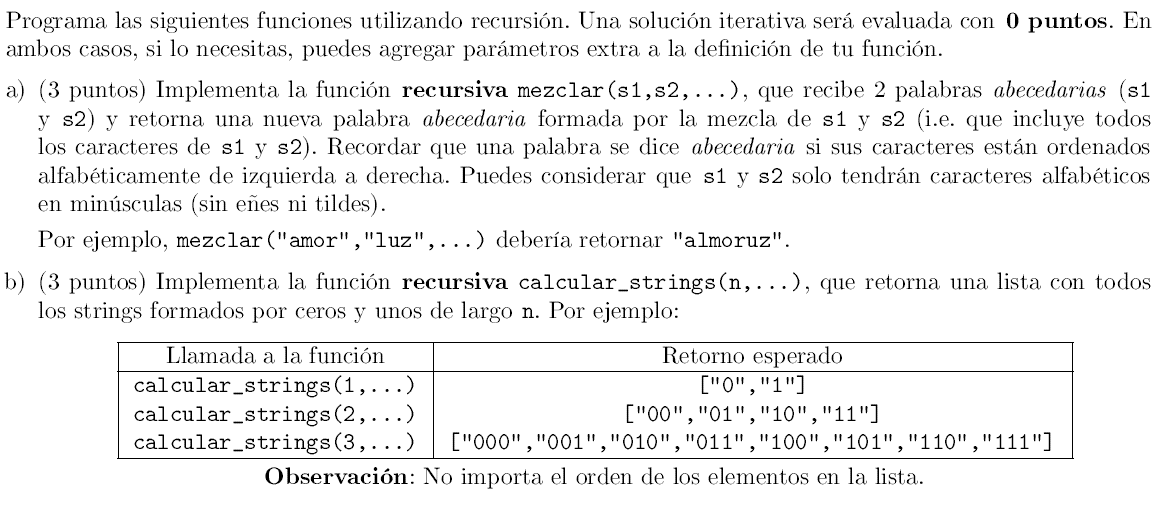
\includegraphics{imgs/pregunta_backtracking.png}
\caption{back1}
\end{figure}

    Una \textbf{posible} solucion de a):

    \begin{Verbatim}[commandchars=\\\{\}]
{\color{incolor}In [{\color{incolor}7}]:} \PY{k}{def} \PY{n+nf}{mezclar}\PY{p}{(}\PY{n}{s1}\PY{p}{,} \PY{n}{s2}\PY{p}{)}\PY{p}{:}
            \PY{k}{if} \PY{n+nb}{len}\PY{p}{(}\PY{n}{s1}\PY{p}{)} \PY{o}{==} \PY{l+m+mi}{0} \PY{o+ow}{and} \PY{n+nb}{len}\PY{p}{(}\PY{n}{s2}\PY{p}{)} \PY{o}{==} \PY{l+m+mi}{0}\PY{p}{:}
                \PY{k}{return} \PY{l+s+s1}{\PYZsq{}}\PY{l+s+s1}{\PYZsq{}}
            \PY{k}{else}\PY{p}{:}
                \PY{k}{if} \PY{n+nb}{len}\PY{p}{(}\PY{n}{s1}\PY{p}{)} \PY{o}{==} \PY{l+m+mi}{0}\PY{p}{:}
                    \PY{k}{return} \PY{n}{s2}\PY{p}{[}\PY{l+m+mi}{0}\PY{p}{]} \PY{o}{+} \PY{n}{mezclar}\PY{p}{(}\PY{n}{s1}\PY{p}{,} \PY{n}{s2}\PY{p}{[}\PY{l+m+mi}{1}\PY{p}{:}\PY{p}{]}\PY{p}{)}
                \PY{k}{elif} \PY{n+nb}{len}\PY{p}{(}\PY{n}{s2}\PY{p}{)} \PY{o}{==} \PY{l+m+mi}{0}\PY{p}{:}
                    \PY{k}{return} \PY{n}{s1}\PY{p}{[}\PY{l+m+mi}{0}\PY{p}{]} \PY{o}{+} \PY{n}{mezclar}\PY{p}{(}\PY{n}{s1}\PY{p}{[}\PY{l+m+mi}{1}\PY{p}{:}\PY{p}{]}\PY{p}{,} \PY{n}{s2}\PY{p}{)}
                \PY{k}{else}\PY{p}{:}
                    \PY{k}{if} \PY{n}{s1}\PY{p}{[}\PY{l+m+mi}{0}\PY{p}{]} \PY{o}{\PYZlt{}} \PY{n}{s2}\PY{p}{[}\PY{l+m+mi}{0}\PY{p}{]}\PY{p}{:}
                        \PY{k}{return} \PY{n}{s1}\PY{p}{[}\PY{l+m+mi}{0}\PY{p}{]} \PY{o}{+} \PY{n}{mezclar}\PY{p}{(}\PY{n}{s1}\PY{p}{[}\PY{l+m+mi}{1}\PY{p}{:}\PY{p}{]}\PY{p}{,} \PY{n}{s2}\PY{p}{)}
                    \PY{k}{else}\PY{p}{:}
                        \PY{k}{return} \PY{n}{s2}\PY{p}{[}\PY{l+m+mi}{0}\PY{p}{]} \PY{o}{+} \PY{n}{mezclar}\PY{p}{(}\PY{n}{s1}\PY{p}{,} \PY{n}{s2}\PY{p}{[}\PY{l+m+mi}{1}\PY{p}{:}\PY{p}{]}\PY{p}{)}
        
        \PY{n+nb}{print}\PY{p}{(}\PY{n}{mezclar}\PY{p}{(}\PY{l+s+s2}{\PYZdq{}}\PY{l+s+s2}{aceg}\PY{l+s+s2}{\PYZdq{}}\PY{p}{,} \PY{l+s+s2}{\PYZdq{}}\PY{l+s+s2}{bdfh}\PY{l+s+s2}{\PYZdq{}}\PY{p}{)}\PY{p}{)}
        \PY{n+nb}{print}\PY{p}{(}\PY{n}{mezclar}\PY{p}{(}\PY{l+s+s2}{\PYZdq{}}\PY{l+s+s2}{amor}\PY{l+s+s2}{\PYZdq{}}\PY{p}{,} \PY{l+s+s2}{\PYZdq{}}\PY{l+s+s2}{luz}\PY{l+s+s2}{\PYZdq{}}\PY{p}{)}\PY{p}{)}
\end{Verbatim}


    \begin{Verbatim}[commandchars=\\\{\}]
abcdefgh
almoruz

    \end{Verbatim}

    Una \textbf{posible} solucion para b)

    \begin{Verbatim}[commandchars=\\\{\}]
{\color{incolor}In [{\color{incolor}13}]:} \PY{k}{def} \PY{n+nf}{calcular\PYZus{}strings}\PY{p}{(}\PY{n}{soluciones}\PY{p}{,} \PY{n}{solucion\PYZus{}parcial}\PY{p}{,} \PY{n}{n}\PY{p}{)}\PY{p}{:}
             \PY{k}{if} \PY{n+nb}{len}\PY{p}{(}\PY{n}{solucion\PYZus{}parcial}\PY{p}{)} \PY{o}{==} \PY{n+nb}{int}\PY{p}{(}\PY{n}{n}\PY{p}{)}\PY{p}{:}
                 \PY{n}{solucion\PYZus{}final} \PY{o}{=} \PY{n}{solucion\PYZus{}parcial}\PY{o}{.}\PY{n}{copy}\PY{p}{(}\PY{p}{)}
                 \PY{n}{aux} \PY{o}{=} \PY{l+s+s1}{\PYZsq{}}\PY{l+s+s1}{\PYZsq{}}\PY{o}{.}\PY{n}{join}\PY{p}{(}\PY{n}{solucion\PYZus{}final}\PY{p}{)}
                 \PY{k}{if} \PY{o+ow}{not} \PY{p}{(}\PY{n}{aux} \PY{o+ow}{in} \PY{n}{soluciones}\PY{p}{)}\PY{p}{:}
                     \PY{n}{soluciones}\PY{o}{.}\PY{n}{append}\PY{p}{(}\PY{n}{aux}\PY{p}{)}
                 \PY{k}{return}
         
             \PY{k}{for} \PY{n}{opcion} \PY{o+ow}{in} \PY{p}{[}\PY{l+s+s1}{\PYZsq{}}\PY{l+s+s1}{0}\PY{l+s+s1}{\PYZsq{}}\PY{p}{,} \PY{l+s+s1}{\PYZsq{}}\PY{l+s+s1}{1}\PY{l+s+s1}{\PYZsq{}}\PY{p}{]}\PY{p}{:}
                 \PY{n}{solucion\PYZus{}parcial}\PY{o}{.}\PY{n}{append}\PY{p}{(}\PY{n}{opcion}\PY{p}{)}
                 \PY{n}{calcular\PYZus{}strings}\PY{p}{(}\PY{n}{soluciones}\PY{p}{,} \PY{n}{solucion\PYZus{}parcial}\PY{p}{,} \PY{n}{n}\PY{p}{)}
                 \PY{n}{solucion\PYZus{}parcial}\PY{o}{.}\PY{n}{pop}\PY{p}{(}\PY{p}{)}
             \PY{k}{return} \PY{n}{soluciones}
         
         
         \PY{k}{for} \PY{n}{i} \PY{o+ow}{in} \PY{n+nb}{range}\PY{p}{(}\PY{l+m+mi}{3}\PY{p}{)}\PY{p}{:}
             \PY{n+nb}{print}\PY{p}{(}\PY{n}{calcular\PYZus{}strings}\PY{p}{(}\PY{p}{[}\PY{p}{]}\PY{p}{,} \PY{p}{[}\PY{p}{]}\PY{p}{,} \PY{n}{i} \PY{o}{+} \PY{l+m+mi}{1}\PY{p}{)}\PY{p}{)}
\end{Verbatim}


    \begin{Verbatim}[commandchars=\\\{\}]
['0', '1']
['00', '01', '10', '11']
['000', '001', '010', '011', '100', '101', '110', '111']

    \end{Verbatim}


    % Add a bibliography block to the postdoc
    
    
    
    \end{document}
